\documentclass[a4paper,fleqn]{cas-dc}
\renewcommand{\printorcid}{}

\usepackage[round]{natbib}
%%%Author definitions
\def\tsc#1{\csdef{#1}{\textsc{\lowercase{#1}}\xspace}}
\tsc{WGM}
\tsc{QE}
\tsc{EP}
\tsc{PMS}
\tsc{BEC}
\tsc{DE}
%%%
\usepackage{booktabs}
\usepackage{array}
\usepackage{microtype}
\begin{document}

\let\WriteBookmarks\relax
\def\floatpagepagefraction{1}
\def\textpagefraction{.001}
\shorttitle{Urban exodus or rural shrinkage?}
\shortauthors{de Graaff, T.}


\title [mode = title]{ Urban exodus or rural shrinkage? Regional migration and attractiveness in a tight Dutch housing market}                      
  \author[1,2]{Thomas de Graaff}[style=dutch, orcid=0000-0002-1782-9742]
  \cormark[1]
  \fnmark[1]
  \ead{t.de.graaff@vu.nl} 
  \ead[url]{www.thomasdegraaff.nl}
\address[1]{Vrije Universiteit Amsterdam}
\address[2]{Tinbergen Institute Amsterdam}

\begin{abstract}
In this paper, I address the impact of home-ownership and social
  renting rates on interregional migration in the Netherlands. I focus
  especially on their relation with natives' migration out of the larger and
  more popular Dutch urban regions. By applying a multilevel social relations model I
  am able to control simultanously for (\emph{i}) both region-specific effects
  of origin and destination, (\emph{ii}) dyad (regional pair) specific effects,
  and (\emph{iii}) the impact of the housing market structure in both the region
  of origin and the region of destination. I find positive and high elasticities
  of social renting ($0.8$) and homeownership ($1.8$) rates on out-migration,
  while homeownership rates have a smaller and negative impact ($-0.5$) on
  in-migration---pointing to the significant role the housing market has on the
  crowding out of natives in the larger urban regions. On top of that, I find that regional
  specific in- and out-migration flows are highly correlated ($0.9$) just as
  regional specific dyadic flows ($0.8$), showing each region's and dyad's
  ideosyncratic migration pattern. Finally, I show that the probabilistic
  model proposed is able to accurately predict migration flows both within and out-of-sample.
\end{abstract}


\begin{keywords}
Gravity model \sep Housing market \sep Interregional migration  \sep multilevel social relations model  \sep Regional Attractiveness
\end{keywords}

\maketitle

\section{Introduction}\label{Introduction}

In the recent decade cities have been proclaimed to be the overall ``winners''
within the regional socio-economic landscape \citep[]{glaeser2012triumph}.
Indeed, there is an abundant empirical literature that finds that especially
large metropolitan areas exhibit---on average---relatively more employment, more
innovation and produce overall more added value \citep[see,
e.g.,][]{balland2020complex}. Most of this success of (large) cities can be
attributed to positive regional and urban agglomeration economies \citep[see for
recent overviews of the size, scope and nature of these urban
economies][]{melo2009meta, duranton2020, rosenthal2020}

Arguably, however, urban benefits do not accrue to everyone equally and recent
empirical research has highlighted the negative sides of the proclaimed urban
success. For example, there is ample empirical evidence of rising levels of
economic segregation witin cities \citep{tammaru2015socio}, of suburbanization
of poverty \citep{hochstenbach2018gentrification}, and crowding out of the
housing market by short-term rentals \citep{koster2018short} and by the
increasing influx of high-skilled migrants to the most popular (inner) cities
\citep{beckers2019residential}.

Indeed, many native residents of large and popular cities are moving out (cite \dots)

Figure \ref{fig:adam_mig} illustrates this by showing out-migration rates of the
urban region of Amsterdam for
various age cohorts in the period 2011--2019. 

\begin{figure}[h!]\centering % Using \begin{figure*} makes the figure take up
  % the entire width of the page
 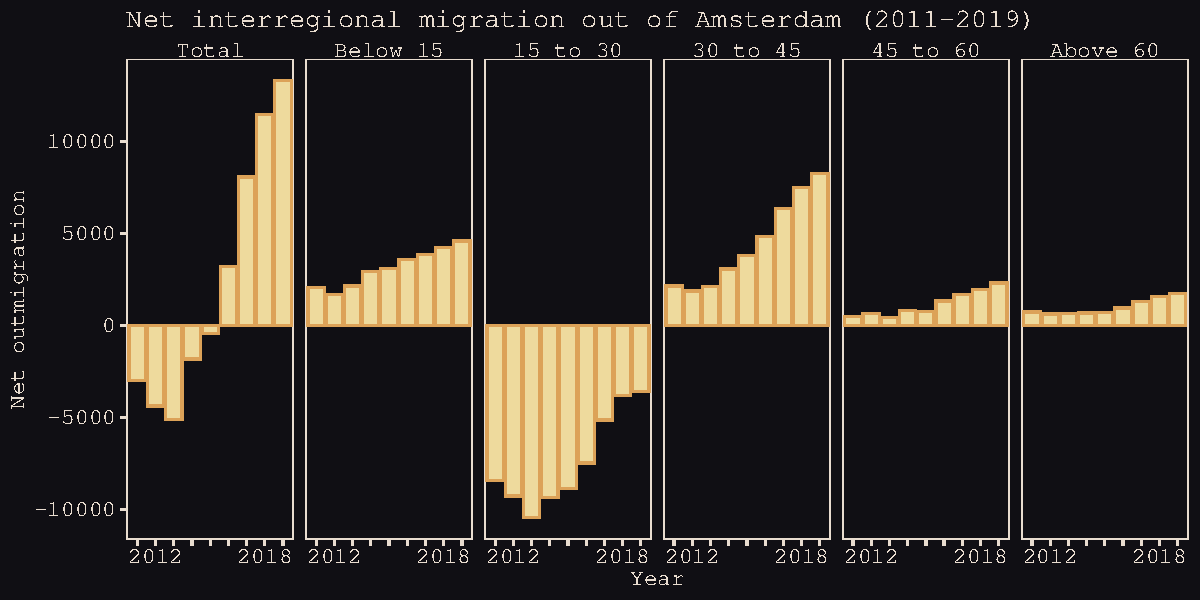
\includegraphics[width=1\linewidth]{../../fig/outmig_amsterdam.pdf}
 \caption{Net regional (domestic) migration into Amsterdam in the period 2011--2020 for
   various age cohorts (including total population in the most left-panel)}
  \label{fig:adam_mig}
\end{figure}

To anticipate the results of this paper, I find strong negative effects of
home-ownership rates on on both in- and out-migration flows. Further, social
renting rates also affect regional migration flows negatively, but only for
out-migration. So, regions accociated with \ldots

This paper reads as follows. The next section describes the data and focuses
especially on the distribution of regional migration flows and housing market
structure. Section 3 describes the modelling approach, where starting from
traditional gravity model and using the descriptives of the migration flows, a
Bayesian multilevel gravity model is constructed. Section 4 gives both the model
results and interprets them by providing as well predictions within and
out-of-sample. The last section concludes.

\section{Literature}

The current Dutch housing market is characterized by a low housing supply
elasticity, high housing demand, and only a small segment (10\%) that belongs to
the private rental market \citep{michielsen2017}. Because of the resulting large
shortage of housing, many policy recommendations have been proposed, including
plans for 700,000 new houses to be built in the coming decade. Unfortunately,
the construction of a large amount of new dwellings is problematic in the
Netherlands due to large and restrictive spatial constraints
\citep{michielsen2019}. Therefore, policy makers consider as well to change the
housing structure, e.g., by converting rent controlled housing to home-ownership
properties, to tackle at least the high housing prices by enlarging the
home-ownership segment.

There is already a large amount of literature looking into the positive and
negative effects of home-ownership---both from a private and from a social
perspective \citep[see for an overview][]{dietz2003social}. It is argued that
home-ownership leads to, e.g., better maintenance (of the own dwelling and the
neighbourhood), more savings, higher education outcomes, higher individual labor
supply, and even better health. One prominent negative effect of home-ownership
is that it leads to less incentives to move residence because of higher moving
costs vis-\`{a}-vis private renting.

This paper revisits the role of housing market structure as impediment for
inter-municipality migration and specifically focuses on the role of
home-ownership and social renting rates. In addition, it gives a framework to
predict changes in the whole network of migration flows, when housing market
structure change locally. To this end, I adopt a Bayesian multilevel gravity
model which is not frequently encountered in the traditional gravity
literature.\footnote{That is, in the economic literature; a notable exception is
  \citet{ranjan2007bayesian} in the economic trade literature. In the
  geographical literature this approach is more commonly adopted \citep[see
  within a migration context][]{congdon2010random, congdon2012spatial}}
Traditional gravity modelling has the disadvantage that either municipality
fixed effects of origins and destinations can be flows. This paper circumvents
this disadvantage by adopting a multilevel incorporated or the municipalities'
characteristics when not varying over approach with partial
pooling\footnote{There is a whole variety of names for these types of models,
  including hierarchical modeling, varying effects, mixed effects and shrinkage
  models. I use the more generic multilevel description as municipality and
  flows are by definition measured at a different level (scale) \citep[see][for
  an indepth discussion]{gelman2013bayesian}.}, where the latter terms indicates
that I do not impose fixed effects to control for origin and destination
specific effects, but that I ``draw'' them from a distribution, hence the name
partial pooling (where complete pooling states no group effects and no pooling
fixed effects).

This papers adds two main elements to the literature. First, it does not only
consider home-ownership but as well municipal social renting structure, which
can be argued \citep[see, e.g.,][]{hughes1981council,
  boyle1997public,boyle1998migration} to have a large effect on regional
mobility as well as social renting rights are usually only valid locally (within
municipality) and are lost when moving residence between municipalities.

Second, a partial pooling approach has another advantage, namely the municipal
varying effects are completely probabilistic, making it feasible to predict both
within and out-of-sample. In other words, with the results at hand I can predict
migration flows between existing \emph{and} hypothetical cities. The former
might be used for looking at counterfactuals; for example, the changes in
in-migration for all municipalities, when one municipality changes its housing
structure. The latter is useful when one wants to assess new migrations flows
between one or even two new municipalities outside the sample.\footnote{See for
  probabilistic predictions of internation migration \cite{azose2015bayesian}.}

That housing market structure has a sizeable effect on migration decisions is
empirically well-established, especially at the micro-level, where it is widely
accepted that home-ownership has a negative effect on municipal mobility
\citep{dietz2003social, dohmen2005housing}. For example,
\citet{palomares2018understanding} find that home-ownership has a very strong
immobility effect on internal migration in Spain during the period 2001--2011.

In the literature, less attention has been given to inter-city migration on the
aggregate level with respect to the housing market as a specific
barrier.\footnote{See \citet{cushing2004crossing} for a historical overview of
  common themes within migration research.} For the UK,
\citet{congdon2010random} found within a multilevel gravity model that social
rented housing had little effect on the attractivity of a region, although it
had a small positive effect on preventing people from moving residence. For the
Canadian case, \citet{amirault2016drags} looked at the impact of home-ownership
on migration flows within a gravity model using a Poisson pseudo maximum
likelihood estimator and found an elasticity around $-1$.

One of the main reasons to look into housing market structure and migration is
that higher moving costs are detrimental to the aggregate labor market
\citep{oswald1996conjecture, oswald1999housing}. There is a large empirical
literature \citep[see, e.g., ][]{munch2006homeowners, munch2008home,
  de2013european} looking at the impact of individual and aggregate
home-ownership on labour market performance, where seemingly paradoxically at
the aggregate level home-ownership is indeed harmful for labour market behaviour
where at the individual level it is correlated with positive labour market
performance.

This difference between individual and aggregate level is explained by sorting.
Home-owners are indeed less mobile than private renters because of higher fixed
and sunk moving costs which has a negative \emph{aggregate} effect on labour
market performance. However, home-owners are different from renters as they do
\emph{individually} better on the labour market (due to individual unobserved
heterogeneity). So home-owners in countries with high home-ownership rates
perform worse on the labour market vis-\`a-vis home-owners in countries with low
home-ownership rates; but they still perform better than private renters. For
social renters, the effect is different from private renters. On the individual
level they are less mobile than renters at the free market as well, but their
labor market performance is also worse than that of private renters
\citep{hughes1981council, de2009homeownership}.

\section{Modeling framework}

\subsection{The traditional gravity model}

In most disciplines, the workhorse model to study aggregate empirical migration
flows has been the gravity model (see \citet{anderson2011gravity} for a generic
survey of the use of gravity models and \citet{poot2016gravity} for an overview
of migration applications). I therefore start by adopting the basic gravity
model specification pioneered by \citet{tinbergen1962shaping}, so:
\begin{equation}
  \text{migrants}_{ij} = \text{M}_i^{\beta_1}\text{M}_j^{\beta_2}\text{dist}_{ij}^\gamma,
  \label{eq:grav}
\end{equation}
where $\text{migrants}_{ij}$ are the number of migrants moving from $i$ to $j$,
$\text{M}_i$ ($\text{M}_j$) denotes the `mass' of $i$ ($j$), and
$\text{dist}_{ij}$ the distance between $i$ and $j$. Usually, the `mass'
variables are proxied by population, gross domestic product, density, etcetera.
Moreover, the variable $\text{dist}_{ij}$ may represent in general all sorts of
frictions, not only physical distance.

Crucially, \citet{anderson2003gravity} argue that origin and destination
specific variables should be incorporated to take into account multilateral
resistance terms. Most often, this is done by log-linearising model
(\ref{eq:grav} and incorporating fixed effects for origins and destinations, as
follows:
\begin{equation}
  \log(\text{migrants}_{ij}) = o_i + d_j +  \gamma\log(\text{dist}_{ij})
  \label{eq:gravfixed}
\end{equation}
Note that now all origin and destination specific variables are absorbed by the
fixed effects $o_i$ and $d_j$ and that only variables affecting the frictions
$(\text{dist}_{ij})$ can be incorporated, which could be cumbersome if one is
especially interested in those variables.\footnote{If there is another variable
  dimension---say, repeated observations over time---then this problem might be
  circumvented. However, this requires enough variation in the data as
  time-invariant variables can still not be taken into account.}$^{,}$\footnote{An
  often applied strategy to overcome this problem is to use differences between
  origin and destination specific variables. Take for example $\Delta h_{ij}$ as
  the difference in home-ownership rates between $i$ and $j$. A disadvantage of
  this approach is that the difference between 10\% and 20\% home-ownership
  rates and the difference between 80\% and 90\% home-ownership rates would be
  valued as the same.}
\begin{figure}[ht]\centering
  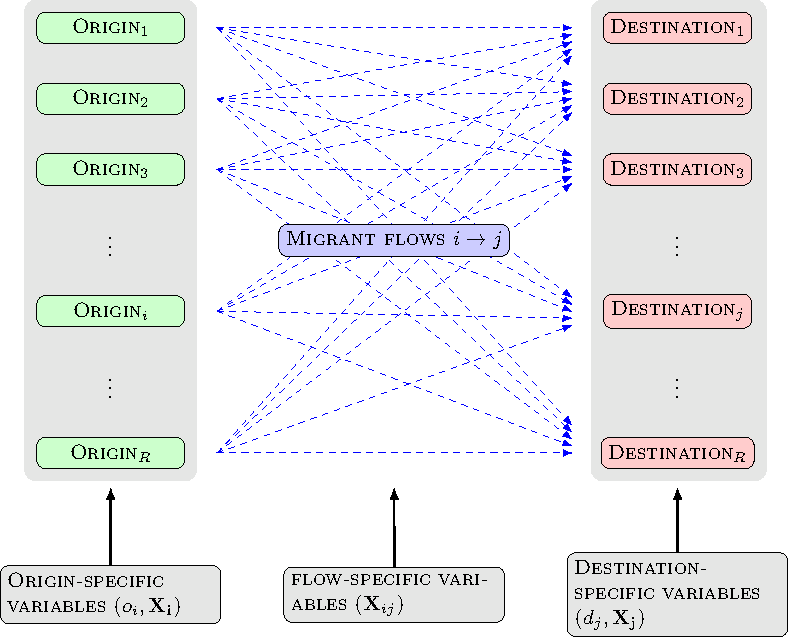
\includegraphics[width=\linewidth]{./../../fig/gravity_network.pdf}
  \caption{Decomposition of variables impacting migration flows from $i$ to $j$
    $\left(\{i,j\} \in \{1,\ldots, R\}\right)$}
  \label{fig:gravity_network}
\end{figure}
Figure \ref{fig:gravity_network} denotes the problem schematically in a generic
dyadic type of network. Typically, one wants to model migration flows between
$i$ and $j$, whilst taken into account both the regional specific effects
($o_i$ and $d_j$) and the regional variables ($\mathbf{X}_i$ and
$\mathbf{X}_j$) one is interested in, such as housing market, population
structure or cultural variables.

Moreover, equation (\ref{eq:gravfixed}) is typically estimated with linear
regression type of models, which is often very cumbersome given the large amount
of zeros migrants flows. `Quick and dirty' remedies as adding a small amount to
the flow variable or removing all zeros have been proven to seriously bias the
results \citep{linders2006estimation, burger2009specification}.

Therefore, I opt in the next subsection for a different strategy, with which I
can tackle simultaneously the two disadvantes of above: incorporating both city
varying effects and city specific variables and modelling the distribution of
migrants flows as they are displayed in Figure \ref{fig:hist_mig_corop}---even when
being zero.

\subsection{A multilevel social relations model for migrants flows}

First, as municipal migrants flows are discrete, non-negative and relatively
rare give the size of the population, theoretically the most appropriate way to
go forward is to model migrant flows with a Poisson type of model. However,
given that the sampling variance is much larger than the sampling mean of the
migration flows (although not conditional on the covariates), we likely need to
correct for overdispersion of heteroskedasticity \citep[][states that
heteroskedasticity (rather than the presence of too many zeros) is responsible
for the main source of bias within gravity models.]{silva2006log}. An often used
distribution to account for overdispersion is the Gamma-Poisson model (which is
under re-parametrization similar to the perhaps better known negative binomial
model). So, we use that for our outcome variable.

To account for the multiplicative nature of the theoretical model as in
(\ref{eq:grav}), I adopt a log link for the expected number of migrants
$\lambda_{ij}$ in the Gamma-Poisson model. Apart from the theoretical model,
note that this log link ensures as well that the expected number of migrants is
always positive. Further, I assume that $\log(\lambda_{ij})$ is a linear
function of the municipal specific variables and the distance between $i$ and
$j$.

Finally, to adopt both municipality effects and variables I adopt a multilevel
model with partial pooling. This entails that the municipal varying effects
(unlike fixed effects) are now drawn from a, in this case Normal, distribution,
where the parameters of this distribution are estimated as well (in the Bayesian
literature they are known as well as hyper-parameters). Intuitively, this
entails that municipalities are partially pooled indicating that (statistical)
information between municipalities is shared. This is an attractive feature, as
fixed effects assume no pooling. In that case, the model only learns from the
information contained in that specific municipality whereas with partial pooling
it is ensured that outliers (very high or low effects) are effectively
\emph{shrunk} towards the mean. Indeed, this is a further extension of that best
feature of linear regression: regression towards the mean.

The complete model now looks as follows:\footnote{I adopt here the model
  structure from \citet{mcelreath2020statistical}.}

\begin{subequations}
  \begin{align} \text{Migrants}_{ij} \sim & \text{Gamma-Poisson}(\lambda_{ij}, \tau) \label{outcome}\\
    \log(\lambda_{ij}) = & \alpha + o_{\text{mun}[i]} + d_{\text{mun}[j]} +
                           \notag \\ & \beta_1 \log(\text{pop}_i) +
                                       \beta_2\log(\text{pop}_j) + \notag \\ &
                                                                               \beta_3
                                                                               \log(\text{home}_i) + \beta_4 \log(\text{home}_j) + \notag\\
                                          & \beta_5 \log(\text{soc}_i) + \beta_6
                                            \log(\text{soc}_j)
                                            + \notag \\ & \beta_7 \log(\text{dist}_{ij}) \label{linear} \\
    d_{\text{mun}} \sim& \text{ Normal}(0, \sigma_d) \label{mund} \\
    o_{\text{mun}} \sim& \text{ Normal}(0, \sigma_o) \label{muno} \\
    \beta_1,\ldots, \beta_7 \sim& \text{
                                  Normal}(0,2)\\ \alpha_o, \alpha_d \sim& \text{ Normal}(0,2)\\
    \sigma_o, \sigma_d \sim& \text{ HalfCauchy}(0,1) \\ \tau \sim& \text{
                                                                   Gamma}(0.01,
                                                                   0.01)
  \end{align}
  \label{model}
\end{subequations}

The first part ({\ref{outcome}) models the outcome variable, being the number of
  migrants, using a Gamma-Poisson distribution (with parameter $\lambda_{ij}$)
  allowing for overdispersion by using an additional parameter $\tau$. The being
  elasticities. Equations (\ref{muno}) and {(\ref{mund}) constitute the linear
    part of the model is given by (\ref{linear}) and states that the poisson
    outcome variable is on a log-scale and that most explanatory variables are
    on a log-scale as well, allowing for direct comparison of the parameters
    multilevel part, where parameters $\sigma_o$ and $\sigma_d$ measures the
    amount of pooling. If they go to zero, then the data exhibits complete
    pooling. If they become very large (go to infinity) there is no pooling
    (which is the fixed effects case). Equations (3e)--(3h) denote priors for
    all parameter involved. These priors are chosen that they are rather
    conservative. Namely, we know from previous empirical literature that the
    $\beta$-parameters typically are not lower than $-2$ or higher than $2$. But
    given the amount of data these priors are of little influence. The only
    structure I impose is that the standard deviations $\sigma_o$ and $\sigma_d$
    are assumed to be non-negative with relatively probability in the their
    right tails. The Gamma prior for $\tau$ is a standard and as well a very
    conservative prior.

\section{Data and methods}

\subsection{Data}

I use inter-regional migration flows measured in individuals between
all of the 40 Dutch COROP regions between 2012 and 2018. I use no information on
within regional migration. So, I have 320 regional
characteristics (or doubled when accounting for both origin and destination
municipalities) and 10,902 aggregate migration flows ($7 \times (40 \times 40 - 40)$).

 \begin{figure}[ht]\centering % Using \begin{figure*} makes the figure take up
% the entire width of the page
   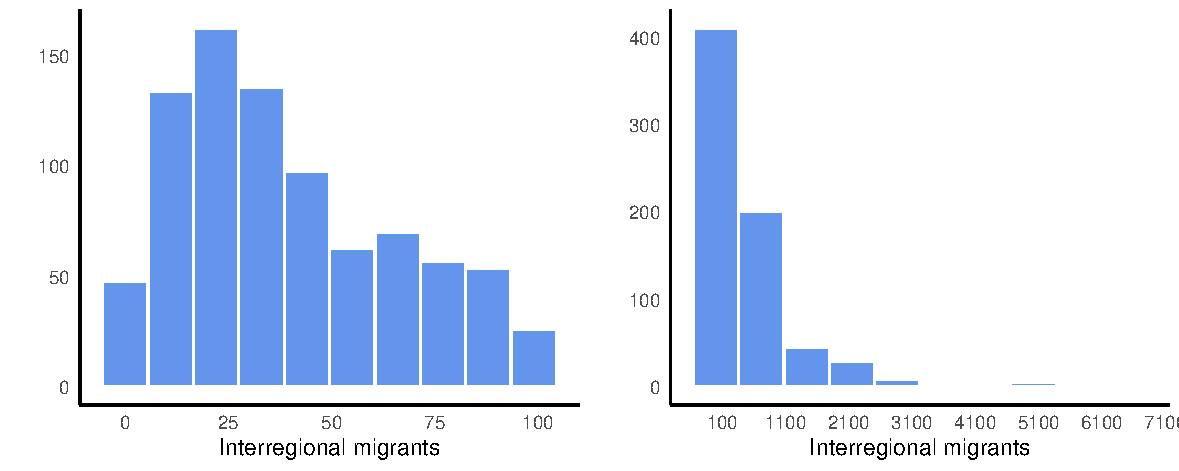
\includegraphics[width=1.0\linewidth]{./../../fig/hist_mig_corop.pdf}
          \caption{Histogram of inter-regional migrant flows. Left panel shows the histogram of
small migrant flows ($0 \leq N < 100$) and the right panel shows the histogram of
large migrant flows ($N \geq 100$). Note the different scale of the y-axes.}
          \label{fig:hist_mig_corop}
        \end{figure}

The histograms in Figure \ref{fig:hist_mig_corop} show the distribution of
migrant flows within my sample. The left panel deals with migrant flows below
100, the right panel with migrant flows of 100 and larger. Two main observations
can be made.

First, there is a strong but consistent decay pattern in migration flow size in
both panels, which points to a persistent underlying pattern. However, the right
`tail' in this distribution is rather thick.\footnote{The largest migration
  flows are between the urban regions of Amsterdam and Utrecht and amount to about
  6,555 migrants in 2018.} Thus, there are still observations quite far right in
the distribution. Indeed, the sample mean is about 270, while the sample
variance is around 290,000, leading to a strong presence of
\emph{overdispersion} (unconditional on other explanatory variables). Second, a
small part of the dataset consists of zero observations. Although they do seem
to be genuine observations and not caused by another process, I check in a
robustness analysis whether the occurrence of zeros does need to be taken
specifically into account.

Seven explanatory variables are added to the model. First, to account for
spatial distance decay between origin $i$ and destination $j$, distance between
all regions are calculated as Eucledian distance between regional centroids
($\text{dist}_{ij}$). Secondly, as regional mass we use population size for
both region of origin and region of destination (so $\text{pop}_i$ and
$\text{pop}_j$). Finally, for housing market structure we use variables
indicating percentage of homeownership ($\text{home}_i$ and $\text{home}_j$) and
percentage of social renting ($\text{soc}_i$ and $\text{soc}_j$), again in both
regions of origin and destination. Social renting in the Netherlands includes all
kinds of rent controlled housing but typically involves local housing
corporations offering housing to lower income households, where eligibility is
based on (local---within region) waiting lists.

\begin{figure}[ht]\centering % Using \begin{figure*} makes the figure take up the entire width of the page
  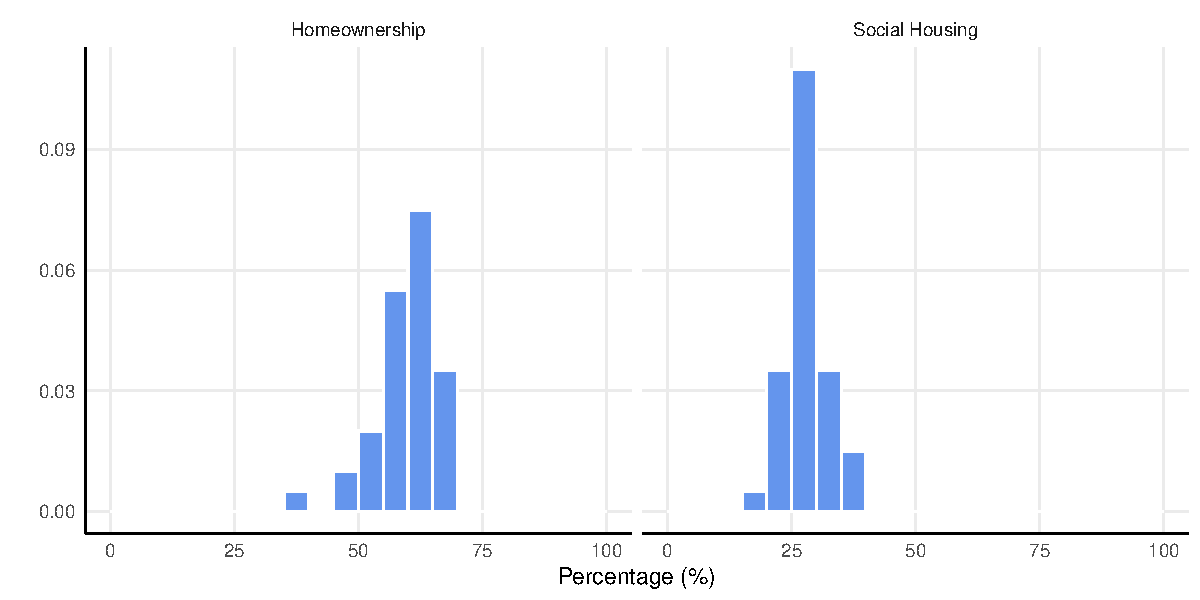
\includegraphics[width=1.0\linewidth]{./../../fig/hist_housing_corop.pdf}
  \caption{Histogram of social housing (left) and homeownership (right)
    percentages in COROP regions in 2018 (check)}
  \label{fig:housing_mig}
\end{figure}

Figure \ref{fig:housing_mig} shows the distribution of social renting and
homeownership across Dutch regions in 2018. Clearly, both home-ownership
and social housing are prevalent across Dutch regions, with an average
per city of 25\% of social housing and around 60\% of homeownership. Moreover, it
is worthwhile to note that social renting is especially prevalent in the larger
cities with a correlation of 0.46 between regional size and social renting (e.g.,
Amsterdam has about a 40\% social renting rate). Also, more rural Dutch regions
exhibit much less social renting. Homeownership and city size
correlate negatively ($-0.63$). Finally, there is a large negative correlation
between social renting and homeownership ($-0.88$) across regions.

\section{Results}

\section{Conclusions}

\section*{Acknowledgments}

I would like to thank Wim Bernasco, Thor Husby, Viktor Venhorst, Maureen
Lanhuizen, participants at the 15$^{\text{th}}$ biennial NECTAR conference in
Helsinki, participants at the 59$^{\text{th}}$ ERSA conference in Lyon and
seminar participants at the VU University Amsterdam for valuable comments on a
first draft of this paper. Paper, data and code can be retrieved from the
following project's GitHub page:

\href{https://github.com/Thdegraaff/migration_gravity}{https://github.com/Thdegraaff/migration\_gravity}.



%%\appendix
%%\section{Appendix}
\section*{Acknowledgements}

\bibliographystyle{cas-model2-names}
\bibliography{references}

\end{document}
